%\documentclass[a4paper,10pt]{jarticle}
%\documentclass[]{jarticle}
\documentclass[10pt]{jarticle}

%\usepackage{graphicx}
\usepackage[dvipdfmx]{graphicx}
\usepackage{eclbkbox} %breakbox用

%本文領域を広め(空白箇所マージン領域を小さめ)に設定
\setlength{\textwidth}{179mm}
\setlength{\textheight}{251mm}
\setlength{\topmargin}{-2cm}
\setlength{\oddsidemargin}{-1cm}
\setlength{\evensidemargin}{-1cm}

\begin{document}

\title{情報工学実験IIレポート(探索アルゴリズム1)}
\author{曜日&グループ番号: 月曜日&グループ0} %
\date{2014年12月14日}

\maketitle

\begin{abstract}
この骨組み(テンプレート)を利用する際には、
不要な箇所を削除した上で提出すること。
例えばこの要旨やコメント文の殆どは
「當間から学生へのコメント」であって、
「課題に対するレポート(報告書)」ではない。

このレポート(ファイル)は、「情報工学実験II・探索アルゴリズムその
1\cite{info2-search1}」の実験レポートの骨組みを例示している。
あくまでも例示であって、全てをこの通りに従う必要はないが、
指示された項目を含めた上で、
報告書として他者が読みやすいレポートとなるよう考慮すること。
\end{abstract}

\section*{グループメンバ}
(補足:レベル毎に \underline{全員が協力して実施} した上で、レベル毎にレポートをまとめる担当者を決め、全体を一つのレポートとして整理すること。分担方法も自由である。)
\begin{itemize}
 \item 945734J 當間愛晃: 担当Level1.1, 1.2
 \item 945700 hoge: 担当Level2.1, 2,2
 \item 945700 hoge: 担当Level2.3, 3.1
 \item 945700 hoge: 担当Level3.2
\end{itemize}

\section*{提出したレポート一式について}
レポート一式は
``\verb|shell:/net/home/teacher/tnal/2013-search1-mon/group0/|''
にアップロードした。
提出したファイルのディレクトリ構成は以下の通りである。

\vspace{+0.5cm}
(補足:必ず下記のように整理しろという指定ではない。
自分たちでやりやすいようにLevel毎に整理しても構わない)
\begin{breakbox}
\begin{verbatim}
./src/      # 作成したプログラム一式
./report/   # レポート関係ファイル.図ファイルを含む.
\end{verbatim}
\end{breakbox}

\newpage

\section{Leve l1: 探索とは}
\subsection{Level1.1: コンピュータと人間の違いを述べよ}
\subsubsection{課題説明}
コンピュータが人間より得意とするモノ、その反対に人間より不得手のモノ、両者について2つ以上の視点(立場や観点など)を示し、考察する。

\subsubsection{考察}
\begin{itemize}
 \item 視点1: hoge\\
コンピュータならば**が可能であり云々
 \item 視点2: fuga\\
人間は**しなくてはならないため云々
\end{itemize}

\subsection{Leve1.2: 評価方法(目的関数の設計指針や方法)について}
\subsubsection{課題説明}
Amazonにおける書籍検索時に「ファンタジー作品で泣ける作品」を探し出すため
のアイテム集合xと目的関数f(x)について検討した。

\subsubsection{アイテム集合xについて}
私達のグループはhogeをfugaすることについて検討を進めた。すなわち云々

\subsubsection{目的関数について}

(補足:PDF図を挿入する例)

%\begin{figure}[h]
% \begin{center}
%  \includegraphics[width=8.0cm]{figs/system-image.pdf}
%  \caption{入出力と内部モデルのイメージ図}
% \end{center}
%\end{figure}



\newpage

\section{Level 2: 最急降下法による最適化}
\subsection{課題説明}
3種類の連続関数$y=x^2$、$z=x^2+y^2$、$y=-x \times sin(x)$について、
最急降下法の適用を通して探索挙動を観察した。
以下ではまず共通部分である最急降下法の探索手続きについて、
フローチャートを用いて解説する。
その後、3種類の関数毎にプログラムの変更箇所、
観察意図観察方法、観察結果、考察について説明する。


\subsection{Level 2共通部分}
(補足:Level2.1, 2.2, 2.3 には共通する部分が多いため、
共通部分は独立して報告すると良いでしょう)

\subsubsection{探索の手続き(共通部分)}

\subsubsection{フローチャート(共通部分)}
(手続きとフローチャートはまとめて一つの節にしても構いません)

 %共通部分の結果及び考察
\subsection{Level2.1: $y=x^2$ について}
\subsubsection{プログラムソース(変更部分)}
\subsubsection{観察意図と観察方法}
\subsubsection{実行結果}
\subsubsection{考察}


\subsection{Level2.2: $z=x^2 + y^2$ について}
\subsubsection{プログラムソース(変更部分)}

	\begin{lstlisting}[caption=探索プログラム,label=ラベル]
	#include <stdio.h>
	#include <stdlib.h>
	#include <math.h>

	-------------省略----------------

	double f(double x, double y) {
  	double z;

  	/** 以下の式を編集して完成させよ(1) **/
  	z = x*x+y*y;

  	return( z );
	}

	/* f(x,y)/dx
 	*    z=f(x,y) の微分値(偏微分値)を求め,返す.
 	*/
	double pd_x(double x, double y) {
  	double z_dx;

  	/** 以下の式を編集して完成させよ(2-1) **/
  	z_dx = 2*x;

  	return( z_dx );
	}

	/* f(x,y)/dy
 	*    z=f(x,y) の微分値(偏微分値)を求め,返す.
 	*/
	double pd_y(double x, double y) {
  	double z_dy;

  	/** 以下の式を編集して完成させよ(2-2) **/
  	z_dy = 2*y;

  	return( z_dy );
	}

	-------------省略----------------

    return 0;
	}
	\end{lstlisting}

\subsubsection{観察意図と観察方法}

\subsubsection{実行結果}
	\begin{lstlisting}[caption=シェルスクリプトalpha.sh実行結果,label=ラベル]
	alpha = 0.01
	FINISH 3 step 643 x and y were not updated.
	sim 1: seed=1000 -> step=642
	FINISH 3 step 712 x and y were not updated.
	sim 2: seed=2000 -> step=711
	FINISH 3 step 697 x and y were not updated.
	sim 3: seed=3000 -> step=696
	FINISH 3 step 702 x and y were not updated.
	sim 4: seed=4000 -> step=701
	FINISH 3 step 717 x and y were not updated.
	sim 5: seed=5000 -> step=716
	FINISH 3 step 690 x and y were not updated.
	sim 6: seed=6000 -> step=689
	FINISH 3 step 688 x and y were not updated.
	sim 7: seed=7000 -> step=687
	FINISH 3 step 701 x and y were not updated.
	sim 8: seed=8000 -> step=700
	FINISH 3 step 701 x and y were not updated.
	sim 9: seed=9000 -> step=700
	FINISH 3 step 714 x and y were not updated.
	sim 10: seed=10000 -> step=713
	average step = 695.50

	-------------省略----------------
	
	alpha = .50
	FINISH 3 step 2 x and y were not updated.
	sim 1: seed=1000 -> step=1
	FINISH 3 step 2 x and y were not updated.
	sim 2: seed=2000 -> step=1
	FINISH 3 step 2 x and y were not updated.
	sim 3: seed=3000 -> step=1
	FINISH 3 step 2 x and y were not updated.
	sim 4: seed=4000 -> step=1
	FINISH 3 step 2 x and y were not updated.
	sim 5: seed=5000 -> step=1
	FINISH 3 step 2 x and y were not updated.
	sim 6: seed=6000 -> step=1
	FINISH 3 step 2 x and y were not updated.
	sim 7: seed=7000 -> step=1
	FINISH 3 step 2 x and y were not updated.
	sim 8: seed=8000 -> step=1
	FINISH 3 step 2 x and y were not updated.
	sim 9: seed=9000 -> step=1
	FINISH 3 step 2 x and y were not updated.
	sim 10: seed=10000 -> step=1
	average step = 1.00

	-------------省略----------------
	
	alpha = .99
	FINISH 3 step 870 x and y were not updated.
	sim 1: seed=1000 -> step=869
	FINISH 3 step 939 x and y were not updated.
	sim 2: seed=2000 -> step=938
	FINISH 3 step 924 x and y were not updated.
	sim 3: seed=3000 -> step=923
	FINISH 3 step 929 x and y were not updated.
	sim 4: seed=4000 -> step=928
	FINISH 3 step 944 x and y were not updated.
	sim 5: seed=5000 -> step=943
	FINISH 3 step 917 x and y were not updated.
	sim 6: seed=6000 -> step=916
	FINISH 3 step 916 x and y were not updated.
	sim 7: seed=7000 -> step=915
	FINISH 3 step 928 x and y were not updated.
	sim 8: seed=8000 -> step=927
	FINISH 3 step 928 x and y were not updated.
	sim 9: seed=9000 -> step=927
	FINISH 3 step 942 x and y were not updated.
	sim 10: seed=10000 -> step=941
	average step = 922.70
	\end{lstlisting}

  \begin{lstlisting}[caption=探索プログラム実行結果,label=ラベル]
  %./steepest_decent2_2 1000 
  step 0 x 0.7557628633 y 2.1064439007 f(x,y) 5.0082834122 5.008283e+00
  step 1 x 0.0000000000 y 0.0000000000 f(x,y) 0.0000000000 0.000000e+00
  FINISH 3 step 2 x and y were not updated.
  \end{lstlisting}
  ※シード値:1000 学習レートα:0.5(最も平均step数が少なかったαの探索結果)

\subsection{Level2.1,2.2 共通部分 考察}

作成したシェルスクリプトalpha.shを実行した結果,当初の予想と同じように学習レートアルファが小さければ詳細に探索でき,アルファが大きくなれば大雑把だが効率よく最適解付近にたどり着くことができることがわかった.今回は,alphaを初期値,刻み幅,最大値をきめ動かしたがしらみつぶしに探索したが,何カ所かの異なるalphaにおいての探索を行うことにより,ある程度効率の良い探索ができる学習レートを予想することができる.

\subsection{Level2.3: $y=-x*sin(x)$ について}
この関数はいくつかの峰と谷を持つ複雑な関数であり,谷を見つけてもそこが最低値かどうかは判断出来ない.そこで以下のようのソースコードを修正した.
\subsubsection{プログラムソース(変更部分)}
\begin{lstlisting}[caption=変更部分,label=fix01]
--------------...
83     n=4;
84     d=X_RANGE/n;
85
86     for (j=0; j < n;j++){
87       x = X_MIN+d*j + (X_RANGE/n) * (double)rand()/RAND_MAX;
...------------
\end{lstlisting}
\subsubsection{観察意図と観察方法}
 これは,最急降下法で観察する部分を分割することで,様々な場所の最小値を発見しようとしている.変更したのは初期値だけであるが,最急降下法は初期値の発生位置によって結果が大きく左右されるため十分であると判断した.観察は当初出力結果を観察していたが,データの推移が判断しにくいためgnuplotでのグラフとの比較を見て判断した.グラフの作成にはシェルスクリプト(スクリプト2.3参照)を用いた.
\subsubsection{実行結果}

\begin{figure}[htb]
 \begin{center}
 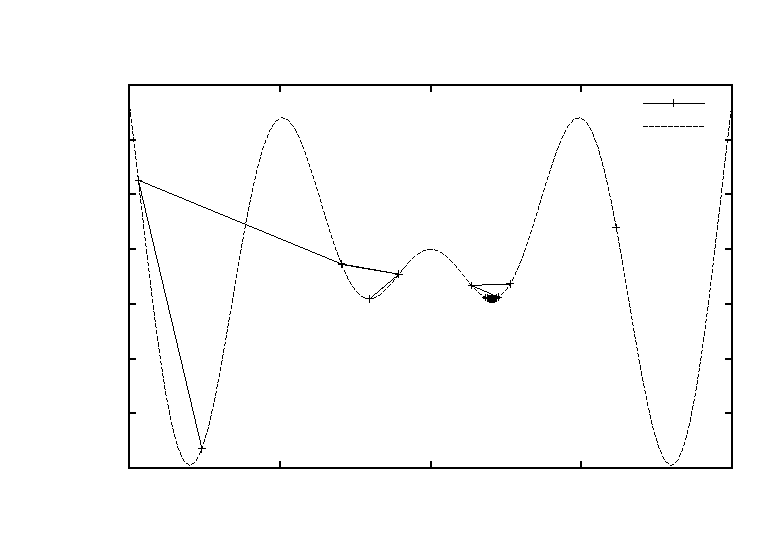
\includegraphics[width=10.0cm]{./level2/level2.3.eps}
  \caption{修正されたプログラムによる出力結果}
  \label{level2.3}
 \end{center}
\end{figure}
\subsubsection{考察}
上の結果が示すように分割した位置で最急降下法を実行することにより,それぞれの谷の位置を発見することが出来た.今回は谷の数を考慮したn(分割数)=4でプログラムを実行したが,現実的にはnもパラメータとして定義し,都合の良い値を推測べきである.



\newpage

\section{Level 3: 最急降下法が苦手とする状況}
\subsection{課題説明}
最急降下法が苦手とする状況についてその理由を解説し、
検討した改善方法について解説する。

\subsubsection{原因}

\subsubsection{改善方法}

 %課題説明+提案解説
\subsection{Level 3.1: $y = x^2 + (y^2)/10$ について}
この関数は1つの谷を持つ関数であるが,最急降下法では上手く最小値を見つける事ができない.
\subsubsection{原因}
最急降下法は勾配ベクトルの逆を進み,山を下るような感覚で最小値を発見しようとするものである.しかし勾配ベクトルには,実際の最小値への方向とは誤差が含まれている.それを刻み値$\alpha$で修正するが,方向にずれが生じているため結果的にジグザグに動くことになる.これは$x$方向と$y$方向の勾配に差があるためであり,結果的には勾配が大きい方に重みが生じていることになる.
\subsubsection{改善方法}
この欠点を改善するためには「共役勾配法」という,前回の進行方向を加味して次の方向を決めるようなアルゴリズムである.これは単純に計算量が増えるものの比較的効率よく最小値を探索することができる.



\subsection{Level 3.2: $y = sqrt(abs(x))$ について}
微分可能ではない解xを含む例。
その理由と、対策手法について検討した。

\subsubsection{原因}
\subsubsection{改善方法}


\newpage

\section{Level 4: モデル推定時における目的関数の設計}
Housing Data Set\cite{housingdata}を例に、
モデルの適切さを図るための目的関数に付いて設計した。

\subsection{目的関数について}
\subsection{設計理由について}


\subsection{Level4.2: 嗜好モデルの構築方法}
\subsubsection{嗜好モデルの説明}
\subsubsection{上記モデルの利点および欠点}





\vspace{+1.0cm}
(補足:参考文献は thebibliography 環境を使って列挙し、
本文中で適切な箇所で引用するようにしましょう。
例えば下記文献は、アブストラクトやLevel 4で引用しています)
\begin{thebibliography}{99}
\bibitem{info2-search1}
情報工学実験2: 探索アルゴリズムその1(當間)\\
\verb|http://www.eva.ie.u-ryukyu.ac.jp/~tnal/2013/info2/search1/|
\bibitem{housingdata}
Housing Data Set\\
\verb|http://archive.ics.uci.edu/ml/datasets/Housing|
\end{thebibliography}

\end{document}
